\documentclass[border=4pt]{standalone}
\usepackage{amsmath,tikz}
\usetikzlibrary{braids,arrows.meta,decorations.markings}
\begin{document}
$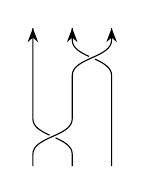
\begin{tikzpicture}[baseline=(current bounding box.center)]
  \pic[draw, yscale=-0.5, braid/width=0.5cm, braid/number of strands=3,
    braid/every strand/.style={postaction={decorate,
      decoration={markings, mark=at position 1 with {\arrow{Stealth[length=5pt]}}}}}]
    (e) {braid={s_1 1 s_2}};
  % \node[below] at (e-1-s) {$X$};
  % \node[below] at (e-2-s) {$Y$};
  % \node[below] at (e-3-s) {$Z$};
  % \node[above] at (e-1-e) {$X$};
  % \node[above] at (e-2-e) {$Y$};
  % \node[above] at (e-3-e) {$Z$};
\end{tikzpicture}
\quad = \quad
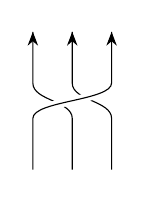
\begin{tikzpicture}[baseline=(current bounding box.center)]
  % Draw Y and Z first, moving the crossing gaps to the hidden X strand.
  \pic[draw, braid/strand 1/.style={draw opacity=0},
    yscale=-0.5, braid/width=0.5cm, braid/number of strands=3,
    braid/every strand/.style={postaction={decorate,
      decoration={markings, mark=at position 1 with {\arrow{Stealth[length=5pt]}}}}}]
    (f) {braid={1 s_1^{-1}-s_2^{-1} 1}};
  % Then overlay X; SVG conversion maps this white underlay to the page background.
  \pic[draw, braid/strand 1/.style={preaction={draw=white, line width=3pt}},
    braid/strand 2/.style={draw opacity=0},
    braid/strand 3/.style={draw opacity=0},
    yscale=-0.5, braid/width=0.5cm, braid/number of strands=3,
    braid/every strand/.style={postaction={decorate,
      decoration={markings, mark=at position 1 with {\arrow{Stealth[length=5pt]}}}}}]
    (e) {braid={1 s_{1,3} 1}};
  % \node[below] at (e-1-s) {$X$};
  % \node[below] at (e-2-s) {$Y$};
  % \node[below] at (e-3-s) {$Z$};
  % \node[above] at (e-1-e) {$X$};
  % \node[above] at (f-2-e) {$Y$};
  % \node[above] at (f-3-e) {$Z$};
\end{tikzpicture}$
\end{document}
